%!TEX root = ../abgabe.tex

\section{Redesign von ''AutoTrader''}

Geschrieben von: \textbf{Hans-Thorben Juilfs}
\newline

In dieser Sektion geht es um ein Fallbeispiel. Das Re-Design und die Entstehung dessen werden beleuchtet und erklärt. Außerdem wird im Folgenden auf einzelne, wichtige Komponenten in der Planung des Designs, sowie der Vorgehensweise eingegangen. Zunächst wird es um die UI-Komponenten(User Interface) gehen.\\

Das Fallbeispiel ist das Re-Design von der iOS app ''AutoTrader'' für Android. Wir haben uns entschieden die im Referat vorgestellte Navigationssoftware nicht noch einmal zu beschreiben, sondern auf eine etwas aktuellere Software zurückzugreifen, um neuere Designaspekte deutlicher ausleuchten zu können.\\

Dabei werden einige Beispiele aufgeführt, die bebildert beschrieben werden und so den Zugang erleichtern.\\

Die vorliegenden Informationen beruhen auf dem Buch ''Android Design Patterns: Interaction Design Solutions for Developers'' von Greg Nudelman\\


\subsection{Logo-Design}
\label{sub:logodesign}
Zunächst wird das Logo und das ensprechende Re-Design beschrieben:\\

\begin{figure}[h]
 \centering
 
\includegraphics[height=0.10\textheight]{img/logo.png}
 \caption{Re-Design des Logos}
 \label{fig:logo}
\end{figure}

Ein Logo wird nach Vorschrift von Apple Inc. immer viereckig, mit abgerundeten Ecken dargestellt. Diese Limitation liegt für Android App-logos nicht vor. Hier wird mehr künstlerische Freiheit gegeben. Um dies zu verdeutlichen wird einfach ein Teil des iOS App-logos genommen und als neues Logo angepasst(siehe Abbildung~\ref{fig:logo}).(\cite{AndroidDesignPatterns} Seite 5)

\subsection{Redesign}
\label{sub:actionbars}

\subparagraph{Vorher}
\label{subp:vorher}
Ersteinmal beschreibt der Autor Greg Nudelman das Aussehen der App bevor das Design angepasst wurde. Hierbei wird aufgezeigt, dass ein großer Knopf mit der Aufschrift ''Settings'' nichts an dem angestammten Platz in der oberen rechten Ecke des Bildschirmes zu suchen hat, da es sich dabei um eine der wichtiges Positionen auf der GUI handelt. Hinzukommt, dass der Knopf keine Einstellungen zeigt, wenn er ausgelöst wurde, sondern lediglich eine ''Anwalts''-Seite zeigt, auf der sich ''Privacy Policy'', ''Visitor Agreement'' und ein Knopf mit der Aufschrift ''Email-Feedback'' befinden(\cite{AndroidDesignPatterns} Seite 6).\\

\begin{figure}[h]
 \centering
 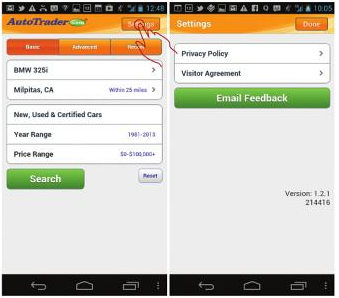
\includegraphics[height=0.40\textheight]{img/Design1.png}
 \caption{Design der GUI1}
 \label{fig:design1}
\end{figure}

Da der ''Settings''-Knopf so einen wichtigen Platz einnimmt, werden wichtigere Funktionen, wie ''Find cars'', ''Find dealer'' oder ''Scan \& Find'' in den Hintegrund gedrängt und sind in einer einem älteren Android nachempfundenen navigation bar menu versteckt. Beides wird in Abbildung~\ref{fig:design1} und Abbildung~\ref{fig:design2} durch eine rote Hand angezeigt.

\begin{figure}[h]
 \centering
 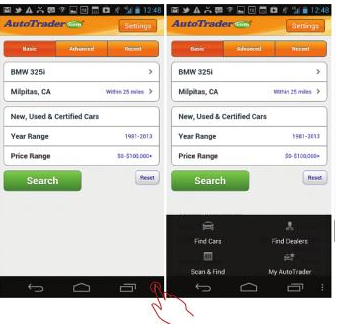
\includegraphics[height=0.40\textheight]{img/Design2.png}
 \caption{Design der GUI2}
 \label{fig:design2}
\end{figure}

\subparagraph{Nachher}
\label{subp:nachher}
Anschließend werden Schritte des Redesigns beschrieben. Zunächst geht Nudelman auf das Umgestalten der o.b. Aspekte, insbesondere den ''Settings''-Knopf und die verstecktion Funktionen ein. In Abbildung~\ref{fig:design3} sind folgende Änderungen zu finden: \\
\begin{itemize}
\item Die Beschriftung des o.g. Knopfes wurde entfernt und durch ein Symbol erseltzt, um ikonische Sprache zu verwenden(\cite{AndroidDesignPatterns} Seite 7). Dies erleichtert die Lokalisation für andere Kulturen, weil nicht übersetzt werden muss. 
\item Der ehemalige Inhalt der navigation bar wurde in die Action bar am oberen Bildschirmrand verschoben und ist so leichter zu finden(\cite{AndroidDesignPatterns}) Seite 7. Dies hilft insbesondere Menschen, welche Schwierigkeiten mit dem Durchsuchen des Bildschirmes nach Funktionen haben. Dabei kann es sich um Blindheit bzw. Sichteinschränkungen oder auch andere, vielleicht psychische Schäden oder Einschränkungen handeln, die ein einfaches Zurechtfinden erschweren.
\end{itemize}

\begin{figure}[h]
 \centering
 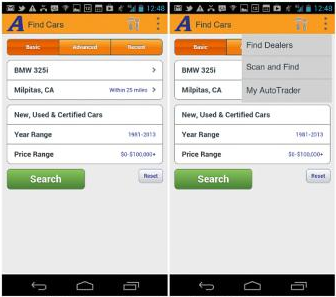
\includegraphics[height=0.40\textheight]{img/Design3.png}
 \caption{Re-Design der GUI1}
 \label{fig:design3}
\end{figure}

Wie Nudelman sagt, wurden aber wichtige Aspekte noch nicht beachtet, während der ersten Umgestaltung. Diese sind:
\begin{itemize}
\item Die Option ''Settings'' ist nicht hilfreich, steht aber durch die prominente Platzierung auf der GUI immernoch über den Funktionen, die im Dropdown menu zu finden wären. Ein Benutzer kommt vermutlich schnell zu dem Schluss, dass die versteckten Funktionen noch weniger hilfreich, als die prominent angeordneten sind und ruft sie daher garnicht erst auf.\\
\item Die wichtigen Optionen werden nicht auf Anhieb gefunden und erfordern daher Suchkapazitäten, die durch den ersten genannten Punkt demotiviert werden(\cite{AndroidDesignPatterns} Seite 8) oder eventuell durch Benutzer mit mentalen oder physischen Herrausforderungen garnicht aufgebracht werden können.\\
\end{itemize}

Diese Aspekte wurden in Abbildung~\ref{fig:design4} beachtet und durch erneute Umgestaltung verwirklicht. Wichtige Funktionen (''Find Dealers'' und ''My AutoTrader'') wurden in die Action bar aufgenommen und ''Settings'' wurde in das Dropdownmenu verschoben(Siehe Abbildung~\ref{fig:design4}).\\

Das sorgt nun für einfaches Auffinden der wichtigsten Optionen und gleichzeitig wird dafür gesorgt den versteckten Funktionen im Dropdown menu nicht die Wichtigkkeit zu nehmen. Somit ist gewährleistet, dass auch den untergeordneten Funktionen Aufmerksamkeit zukommt.\\

\begin{figure}[h]
 \centering
 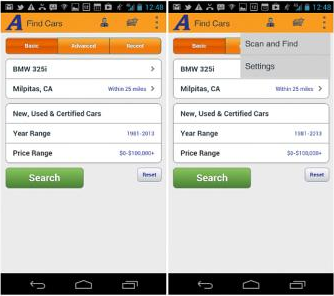
\includegraphics[height=0.40\textheight]{img/Design4.png}
 \caption{Re-Design der GUI2}
 \label{fig:design4}
\end{figure}

\subparagraph{Tabs}
\label{sub:tabs}

Als nächstes werden die Tabs umgestaltet. Leider findet man eine kleine Unzulänglichkeit in dem neuen Design, auf die später eingegangen wird. Grundlegend wird aus aneinander ''klebenden'' Knöpfen ein einheitliches Design geschaffen und anstatt den gesamten Knopf farbig zu Kennzeichnen wird ein Balken unter der Beschriftung angezeigt, um aufzuzeigen, welches Tab aktiv ist(Siehe Abbildung~\ref{fig:tabs}). Nebenbei wird erwähnt, dass ein verkleinertes Display zur Folge hat, dass die in den unteren Tabs gezeigte Schrift dann in Symbole gewandelt wird, um die Übersicht zu gewährleisten(\cite{AndroidDesignPatterns} Seite 11).\\

Die kurz erwähnte Schwachstelle ist das eben schon genannte Anzeigen des aktiven Tabs durch einen Balken unter dem Text des aktiven Tabs. Hierdurch verringert sich der wahrnehmbare Bereich, was wiederrum zur Folge hat, dass Menschen mit geringerer Sehkraft ihn unter Umständen nicht wahrnehmen können. Dies kann zu Verwirrung führen.\\

\begin{figure}[h]
 \centering
 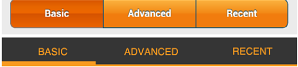
\includegraphics[height=0.08\textheight]{img/tabs.png}
 \caption{Re-Design der Tabs}
 \label{fig:tabs}
\end{figure}

\subparagraph{Selektion}
\label{sub:selection}
Ein weiteres Umgestalten fand an der Selektion eines zu beschauenden Autos statt. Vor der Umgestaltung gab es ein für iOS-Apps übliches Design, dass durch kleine Pfeile an einer Seite indizierte, dass durch Auswahl des entsprechenden Bereiches weitere Informationen angezeigt werden(Siehe Abbildung~\ref{fig:selection} oben). Nach Nudelman ist es unter Android OS üblich, dass das Konzept ''Tap Anywhere'' ausgeprägt gelebt wird(\cite{AndroidDesignPatterns} Seite12). Daraus folgt, dass keine visuellen Hinweise zu den weiteren Informationen führen(Siehe Abbildung~\ref{fig:selection} unten).\\

Dieses Einsparen visueller Hinweise hat zur Folge, dass der Informationsgehalt der GUI zurückgeht. Daher ist auch hier ein Problem zu erkennen: Sollte der Benutzer sich nicht mit dem erwähnten gelebten Konzept auskennen, wird unter Umständen die zusätzlich verfügbare Information nicht gefunden.\\
\begin{figure}[h]
 \centering
 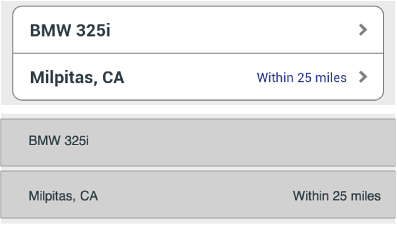
\includegraphics[height=0.08\textheight]{img/rows.png}
 \caption{Re-Design der Selection Page}
 \label{fig:selection}
\end{figure}

\subparagraph{Suche}
\label{sub:search}
Neben den genannten Änderungen wird in \cite{AndroidDesignPatterns} Seite 15 beschrieben, wie die Suchoption angepasst wurde. Aus einem links angeordneten Knopf für die Suche und einem kleinen rechts angeordneten Knopf zum Zurücksetzen der Suche(Siehe Abbildung~\ref{fig:search} oben) werden nach der Umgestaltung zwei unterschiedlich breite, aber gleich hohe Tippfelder, die die gesamte Bildschirmbreite ausfüllen(Siehe Abbildung~\ref{fig:search} unten).\\

Hier gibt es einen deutlichen Vorteil durch das neue Design: Die Suche befindet sich nun auf der rechten Seite und da die meisten Menschen(ca. 90\%, siehe \cite{Handedness}) Rechtshänder sind, wird durch dieses Design auf einen größeren Teil der potentiellen Benutzer Rücksicht bezüglich des Komfort bei der Bedienung genommen. Dadurch, dass das Tippfeld für die Suche mehr als die Hälfte der Bildschirmbreite einnimmt, ist es für Linkshänder kein deutlicher Nachteil in der Bedienung.

\begin{figure}[h]
 \centering
 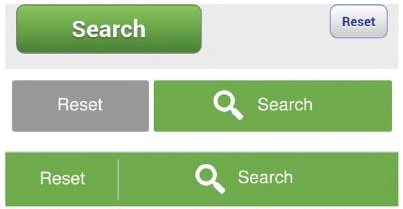
\includegraphics[height=0.08\textheight]{img/search.png}
 \caption{Re-Design der Suche}
 \label{fig:search}
\end{figure}